% ----------------------------------------------------------
% Desenvolvimento
% ----------------------------------------------------------
\chapter{Desenvolvimento}
\label{cap:desenvolvimento}
% ----------------------------------------------------------
A proposta da ferramenta é permitir que o aluno explore o funcionamento de um APN, com clareza a respeito do seu não determinismo. Adicionalmente, queremos que o aluno seja capaz de testar a corretude de um autômato. Este último passo requer uma especificação da linguagem que o APD deve aceitar. Para tanto, empregamos GLCs como uma forma de especificar a linguagem a ser implementada.

O processo de correção automatizado consiste na geração de palavras que devem ser aceitas pelo APD. Para esta etapa, empregamos o uso de um método baseado em derivadas livres de contexto.

Este capítulo apresenta como a ferramenta foi desenvolvida e descreve a arquitetura de software utilizada, assim como as bibliotecas e técnicas de programação. Ele está organizado da seguinte forma: a seção \ref{sec:impl} descreve a implementação da ferramenta; a subseção \ref{sec:rpl} descreve de forma geral como o APD e sua execução foram modelados; por fim, a seção \ref{sec:gen} apresenta a implementação do gerador de palavras a partir de uma dada GLC.


\section{Implementação}\label{sec:impl}

A ferramenta foi desenvolvida utilizando a linguagem de programação JavaScript, com foco na orientação a objetos, com o auxílio de HTML5 e CSS para a sua apresentação visual. A aplicação ocorre completamente no \emph{front-end} e não possui partes executadas em servidor. Também não foi utilizado nenhum tipo de \emph{framework} para auxiliar na organização do código. Além das tecnologias nativas, foi utilizada a biblioteca JavaScript Cytoscape.

A biblioteca Cytoscape é utilizada para a manipulação de desenhos em HTML5, com foco na visualização de grafos. Ela foi escolhida por ser totalmente \emph{open source} e porque grafos são a forma mais comum de representação de autômatos, utilizada, por exemplo, no livro didático \cite{vieira2006}. A biblioteca foi empregada apenas para o desenho dos grafos, tendo toda a parte de simulação de autômatos sido desenvolvida exclusivamente durante este trabalho. O código-fonte está disponível no GitHub, e o software encontra-se hospedado de forma gratuita por meio do GitHub Pages para testes.

O sistema desenvolvido originalmente possuía os seis tipos de máquinas de estados estudados na disciplina de Fundamentos Teóricos da Computação na UFOP. Porém, devido ao tempo limitado e ao escopo abrangente, foi tomada a decisão de seguir apenas com a representação de APNs e a correção de exercícios. Caso haja interesse, essa versão beta pode ser encontrada \href{https://matheushvribeiro.github.io/simulador-de-automatos/index.html}{neste repositório}, ao passo que o código mais recente está disponível \href{https://github.com/lives-group/APN-simulator}{neste repositório}.

\subsection{Modelagem do APD e sua execução}
\label{sec:rpl}
\subsection{Modelagem do APD e sua execução}
\label{sec:rpl}

Ao desenvolver este projeto, foi feita uma divisão entre a representação lógica e a representação gráfica do APN. A representação lógica do APN e a sua execução dentro do sistema acontecem por meio de quatro classes principais: \texttt{Transition}, \texttt{APN}, \texttt{Snapshot} e \texttt{APNRunner}. Ao passo que as classes \texttt{Transition} e \texttt{APN} descrevem os aspectos estáticos do autômato, as classes \texttt{Snapshot} e \texttt{APNRunner} são usadas para emular o comportamento do autômato sobre uma dada entrada.

Cada transição foi representada utilizando objetos da classe \texttt{Transition}, que possui quatro atributos simples: \texttt{sym}, que é o caractere a ser lido na palavra; \texttt{stkR}, que é o valor que deverá ser desempilhado da pilha; \texttt{stkW}, que é o valor que deverá ser empilhado na pilha; e o atributo \texttt{state}, que é o estado de destino daquela transição.

A classe \texttt{APN} ficou responsável por reunir os estados e as transições, além de alguns métodos auxiliares. Essa classe contém os seguintes campos privados:
\begin{itemize}
   \item \texttt{\#states}: Uma lista de estados. Cada estado é representado por um valor numérico.
   \item \texttt{\#transitions}: Um mapa que associa a cada estado, uma lista de objetos que representam transições.
   \item \texttt{\#finals}: Uma lista de estados finais.
   \item \texttt{\#start}: Uma lista de estados iniciais.
\end{itemize}

O método \texttt{addState(s)} permite adicionar um novo estado, desde que \texttt{s} seja um número e já não esteja presente no conjunto de estados. A função \texttt{removeState(s)} procura por um estado e o remove da lista de estados, observando a necessidade de se atualizar a lista de transições de todos os demais estados, a lista de estados finais e iniciais. A função \texttt{addTransition(s,t)} adiciona um objeto de transição \texttt{t} à lista de transições de \texttt{s}. A função \texttt{removeTransition(s,t)} remove o objeto de transição cuja referência é dada por \texttt{t} da lista de transições do estado \texttt{s}. Além desses métodos, há métodos para setar e obter estados iniciais e finais. Tais métodos são triviais (e bem documentados na implementação).

A classe \texttt{APN} possui ainda, o método \texttt{delta}, que utiliza os atributos do seu mapa de transições para determinar quais transições podem ser atingidas a partir de um estado $s$, um caractere de palavra $chr$ e um topo de pilha $r$, retornando esse conjunto de transições na forma de um \emph{array}. Esse método percorre cada transição que tem sua chave no mapa igual a $s$ (já que sua chave no mapa é seu estado de origem) e, em cada uma, verifica se o atributo \texttt{sym} é igual a $chr$ ou à string vazia, e se o atributo \texttt{stkR} é igual a $r$ ou à string vazia. Se ambas as condições forem satisfeitas simultaneamente, essa transição é considerada válida e é adicionada ao \emph{array} que será retornado ao final do método.

O maior desafio ao representar APNs neste projeto foi modelar o seu não determinismo, dado que existem muitas execuções simultâneas do mesmo autômato. A forma adotada para representar cada uma das execuções simultâneas causadas pelo não determinismo foi a criação da classe \texttt{Snapshot}, na qual cada \texttt{Snapshot} representa um ponto da execução de um dos possíveis caminhos da máquina, podendo vários \texttt{Snapshots} existir simultaneamente.

Para modelar isso, a classe \texttt{Snapshot} conta com os seguintes atributos: \texttt{state}, que representa o estado em que a execução se encontra; \texttt{pos}, que representa a posição do caractere lido na palavra que está sendo processada; e \texttt{stack}, que representa o array com o conteúdo da pilha naquele momento da execução. Além de armazenar os dados, a classe \texttt{Snapshot} dispõe de métodos utilitários essenciais, como o \texttt{top()}, que retorna o valor atual no topo da pilha (ou a \emph{string} vazia, caso não haja elementos), e o método \texttt{equal(snp)}, que realiza a comparação profunda de conteúdo entre duas instâncias, garantindo que configurações instantâneas sejam consideradas idênticas apenas se possuírem o mesmo estado, a mesma posição de leitura e o mesmo arranjo na pilha.

Para a visualização do usuário, é criado um grafo de \emph{snapshots} construído na classe \texttt{Graph}. Essa classe pode ser utilizada para a criação de grafos de qualquer tipo de objeto JavaScript, sendo composta por dois mapas: um que tem como chave um ID e como valor um único objeto que representa um nó; e um segundo mapa, que representa as arestas entre os nós utilizando os valores de ID do primeiro mapa, no qual a chave é o nó de origem e o valor é o nó de destino da aresta.

A classe \texttt{APNRunner} é a principal responsável por emular o comportamento dinâmico do autômato sobre uma dada entrada. Esta classe contém os seguintes campos privados principais:
\begin{itemize}
   \item \texttt{\#apn}: Um objeto da classe \texttt{APN} que será executado.
   \item \texttt{\#input}: A palavra (cadeia de caracteres) que será processada.
   \item \texttt{\#snaps}: Um \emph{array} de objetos da classe \texttt{Snapshot}, armazenando as configurações instantâneas atuais.
   \item \texttt{\#graph}: O grafo rastreador da execução, construído para visualização.
   \item \texttt{\#accType}: O tipo de critério de aceitação esperado (\texttt{'F'}, \texttt{'S'} ou \texttt{'FS'}).
   \item \texttt{\#limit}: O limite de \emph{loops} estipulado para a simulação, prevenindo execuções infinitas.
\end{itemize}

Na sua inicialização, por meio do método \texttt{start()}, a classe prepara a simulação iterando sobre os estados iniciais do autômato para instanciar os \emph{snapshots} de partida, registrando-os imediatamente como os primeiros nós no grafo.

O principal método encarregado de avançar a execução é o \texttt{step}. Ele percorre cada um dos \emph{snapshots} atuais e verifica as transições válidas a partir deles por meio do método \texttt{delta} da classe \texttt{APN}. Para processar a mudança de estado e manipular a pilha, o \texttt{step} utiliza a função auxiliar \texttt{transition(t, snp)}. Essa função recebe um objeto de transição e um \emph{snapshot}, verifica se a regra consome um caractere da palavra (ou se é uma transição vazia) e, se aplicável, gera um novo \emph{snapshot} devidamente atualizado — desempilhando e empilhando os símbolos definidos pela transição e avançando o ponteiro de leitura da entrada. As transições válidas resultantes passam a ser os \emph{snapshots} atuais e são adicionadas ao grafo, criando-se uma aresta entre cada \emph{snapshot} original e os gerados a partir dele.

A simulação acontece por meio do método \texttt{runUntilAcc()}, que realiza sucessivas chamadas à função \texttt{step} até que uma de três condições de parada seja atingida: (I) todos os caminhos possíveis se esgotam (\emph{snapshots} atuais ficam vazios); (II) o limite de \emph{loops} de execução definido pelo usuário é atingido; ou (III) a palavra é aceita. Alternativamente, a execução pode ser controlada passo a passo através do método \texttt{next()}.

Por fim, a verificação de aceitação da palavra é flexível e feita a cada etapa. A classe \texttt{APNRunner} oferece três métodos distintos baseados na propriedade \texttt{accType}: o método \texttt{acceptedF()}, que verifica se algum \emph{snapshot} concluiu a leitura da palavra e parou em um estado final; o \texttt{acceptedS()}, que checa se a palavra foi totalmente lida e a pilha se encontra vazia; e o \texttt{acceptedFS()}, que exige rigorosamente a satisfação de ambas as condições simultaneamente.

\subsubsection{Exemplo de Uso: Linguagem $a^n b^n$}

Para ilustrar o funcionamento integrado dessas classes, apresenta-se a seguir a instanciação de um Autômato de Pilha (neste caso, determinístico) projetado para reconhecer a linguagem $L = \{a^n b^n \mid n > 0\}$. O autômato possui três estados: o estado 0 empilha o caractere `A` ao ler o primeiro `a`; o estado 1 continua empilhando `A` para leituras subsequentes de `a` e transita para o estado 2 ao ler o primeiro `b` (desempilhando); e o estado 2 continua desempilhando ao ler o caractere `b`. A aceitação ocorre por estado final (2) e pilha vazia (\texttt{FS}).

O fragmento de código em JavaScript a seguir demonstra a construção da lógica e o laço para a sua execução passo a passo utilizando o método \texttt{next()}:

\begin{lstlisting}[language=javascript]
import { APN, Transition, APNRunner } from './APN.js';

// 1. Criação do autômato e definição dos estados
let apn = new APN();
apn.addState(0);
apn.addState(1);
apn.addState(2);

apn.addInitialState(0);
apn.addFinalState(2);

// 2. Definição das transições
// Estado 0: Lê o primeiro 'a', empilha 'A' e vai para o estado 1
apn.addTransition(0, new Transition('a', '', ['A'], 1));

// Estado 1: Lê 'a' adicionais, empilha 'A' e continua no 1
apn.addTransition(1, new Transition('a', '', ['A'], 1));

// Estado 1: Lê o primeiro 'b', desempilha 'A' e vai para o estado 2
apn.addTransition(1, new Transition('b', 'A', [], 2));

// Estado 2: Lê 'b' adicionais, desempilha 'A' e continua no 2
apn.addTransition(2, new Transition('b', 'A', [], 2));

// 3. Configuração da execução
let input = "aabb";
let accType = "FS"; // Aceitação por Estado Final e Pilha Vazia
let limit = 20;

let runner = new APNRunner(apn, input, accType, limit);
console.log("Iniciando execução para a palavra: " + input);

// 4. Laço de execução passo a passo
while (!runner.exausted() && !runner.acceptedFS()) {
    runner.next();
    // Imprime o estado das configurações atuais e passadas
    console.log(runner.lastStepString());
}
// 5. Verificação do critério de aceitação
if (runner.acceptedFS()) {
    console.log("Palavra aceita pelo autômato!");
} else {
    console.log("Palavra rejeitada!");
}
\end{lstlisting}

\subsection{Gerando palavras a partir de uma GLC}\label{sec:gen}

O processo para geração de palavras consiste no uso de derivadas para sintetizar uma palavra a partir de uma GLC. Essa abordagem é simples e tem a vantagem de garantir, por definição, que a palavra sintetizada deverá necessariamente ser aceita por qualquer APN que implemente a respectiva GLC. A técnica consiste em, iterativamente, derivar a GLC em relação a um símbolo proveniente do conjunto \emph{First} do símbolo de partida. A cada passo, inspecionamos se o símbolo de partida é anulável; em caso afirmativo, a concatenação de todos os símbolos derivados até o momento forma uma palavra de entrada válida que deve ser aceita pelo APN.

Intuitivamente, o conjunto \emph{First}, frequentemente empregado em reconhecedores sintáticos LL(1) \cite{Aho2006}, pode ser entendido como o conjunto de todos os símbolos terminais que podem ser produzidos imediatamente por uma forma sentencial. Por exemplo, uma regra na forma $A \to aAb \;|\; c$ possui como conjunto \emph{First} os elementos $\{a,c\}$. Dada uma gramática $G = \langle \Sigma, V, R, P \rangle$, seja $F(A)$ o conjunto \emph{First} do não terminal $A$. Inicialmente, para cada $A \in V$, $F(A) = \emptyset$. Formalmente, o conjunto \emph{First(X)} pode ser definido pela aplicação das seguintes regras, repetidas até que nenhum dos conjuntos sofra alterações:

  \begin{enumerate}
   \item Se $X$ é um terminal, então $First(X) = \{X\}$.
   \item Se $X$ é um não terminal com regra $X \to Y_1\,Y_2\,\ldots\,Y_k$ (para algum $k \geq 1$), e se existe algum $j$ tal que $\neg nullable(Y_j)$ com $0 \leq j \leq k$, então $First(X) = First(X) \cup First(Y_i)$ para $0 \leq i \leq j$.
  \end{enumerate}

O conjunto de não terminais anuláveis (\emph{nullables}) de uma GLC é o conjunto de todos os não terminais que podem gerar a palavra vazia ($\epsilon$). Esse conjunto pode ser computado pela aplicação das seguintes regras até que o conjunto pare de mudar:

  \begin{enumerate}
     \item Para toda produção na forma $A \to \epsilon$, temos que $A \in \,nullables$.
     \item Para toda produção na forma $A \to B_1\,\ldots B_n$, se $B_1\,\ldots B_n \in nullables$, então $A \in nullables$.
  \end{enumerate}

A implementação desses conceitos em JavaScript se beneficia do uso do tipo de dados \texttt{Set} para a implementação de \emph{nullables}, e de \texttt{Map} para a implementação do \emph{First}. Esses conceitos foram codificados em uma classe que modela uma GLC, formada por um \texttt{Map} que armazena as produções da gramática. A API desenvolvida permite a adição de regras e a definição do símbolo de partida, além de disponibilizar o método \texttt{derivate}, que cria uma cópia da gramática contendo as regras derivadas.

A implementação do método da derivada também copia a tabela \emph{First} da gramática original. Como o \emph{First} é computado por um algoritmo de ponto fixo e todas as produções da gramática base são copiadas para a derivada, o novo conjunto \emph{First} não precisa ser computado do zero, baseando-se no conjunto original. Isso permite que apenas adicionemos à tabela as novas produções mais relevantes. A API da gramática contém ainda o método \texttt{prune}, responsável por remover produções inatingíveis a partir do símbolo de partida.

Finalmente, o processo para a geração de uma palavra pode ser descrito pela seguinte sequência de passos, dada a gramática $G = \langle \Sigma, V, R, P\rangle$:

  \begin{enumerate}
     \item Inicialize a palavra $w$ com $\epsilon$.
     \item Inicialize o conjunto $WRDS$ com $\emptyset$.
     \item \label{gen:inicio} Se $P$ pode gerar $\epsilon$, faça $WRDS = WRDS \cup \{w\}$.
     \item Compute o \emph{First($P$)}.
     \item Escolha, aleatoriamente, um símbolo $a$ de \emph{First($P$)}.
     \item Compute a derivada de $G$ em relação a $a$.
     \item Remova as produções inatingíveis de $G$.
     \item Atualize a lista de produções anuláveis.
     \item Retorne ao passo \ref{gen:inicio}.
  \end{enumerate}

\section{Uso do software}\label{sec:uso}

A interface do software pode ser dividida em duas partes principais: criação/edição de APNs e execução do APN com base em uma palavra. A parte de criação permite: instanciar estados; editar o nome do estado; defini-lo como final, inicial, ambos ou nenhum; excluí-lo; criar transições; editar valores da transição; excluir transições; baixar o APN desenvolvido; importar um APN desenvolvido anteriormente; mover livremente os elementos; e aplicar \emph{layouts} prontos do Cytoscape para organizar a visualização.

Já a parte de execução do APN permite: definir a palavra de entrada; estipular o número limite de \emph{loops} para a função \texttt{step}; escolher a condição de aceitação entre FS (estado final e pilha vazia), S (pilha vazia) ou F (estado final); iniciar e interromper a simulação; avançar ou retroceder um \texttt{step}; reiniciar a execução; e visualizar os dados completos de cada \emph{snapshot} individualmente ao clicar nele.

Para exemplificar a utilização, vamos ao cenário de um autômato simples. Para criar cada estado na ferramenta, basta clicar no painel esquerdo do sistema, conforme a Figura~\ref{img:createState}. Clicando em um estado com o botão direito, abrem-se as opções de edição: "inicial" e "final" (que alternam o estado daquele nó), além de "renomear" e "excluir". Essas funções são ilustradas na Figura~\ref{img:editState}.

    \begin{figure}[h]
        \begin{subfigure}{0.5\textwidth}
           \centering
           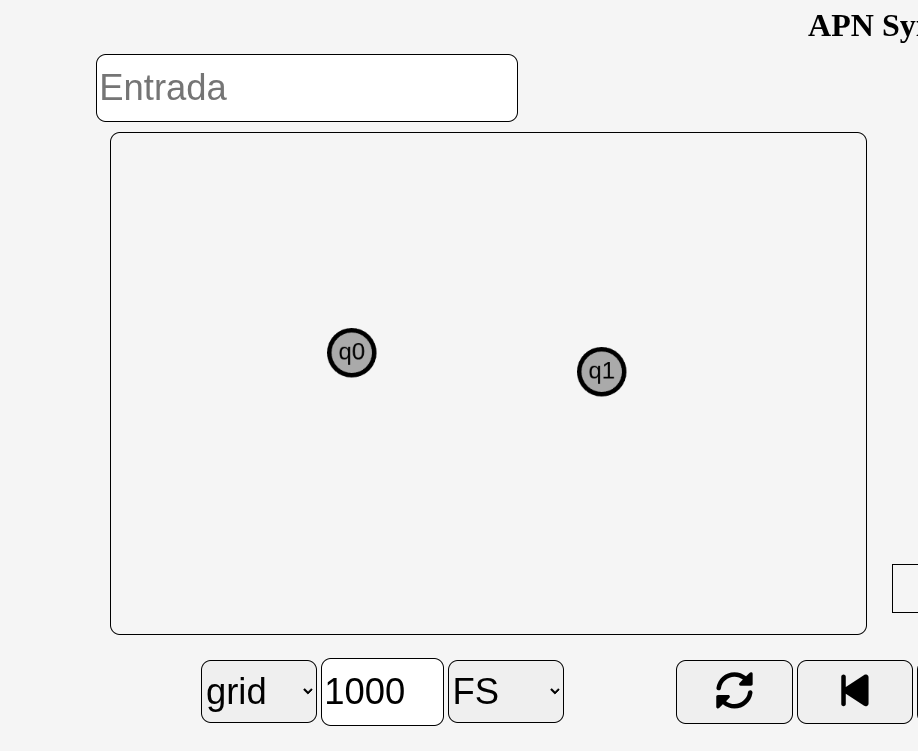
\includegraphics[scale=.24]{img/createState.png}
           \caption{}\label{img:createState}
        \end{subfigure}
        \begin{subfigure}{0.5\textwidth}
           \centering
           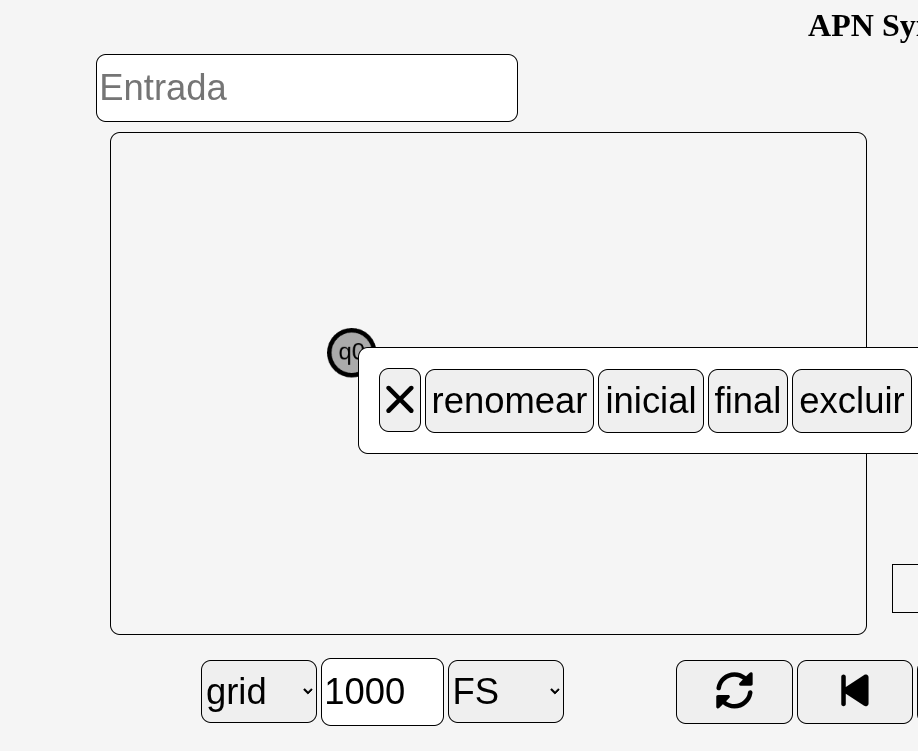
\includegraphics[scale=.24]{img/editState.png}
           \caption{}\label{img:editState}
        \end{subfigure}
        \caption{\subref{img:createState} Criação do estado, \subref{img:editState} Editando o estado }
    \end{figure}

Para criar uma transição, clique no estado de origem com o botão esquerdo e, em seguida, no estado de destino. A transição gerada tem, por padrão, o valor $\lambda$ em todos os elementos, como mostra a Figura~\ref{img:createTransition}. Ao clicar em uma transição com o botão direito, suas opções de edição são exibidas (Figura~\ref{img:editTransition}): "excluir" e "renomear", que permite alterar o caractere de leitura, o caractere a ser desempilhado e o caractere a ser empilhado, caso deixado em branco o campo será considerado como $\lambda$. Um exemplo de autômato simples construído na ferramenta pode ser visto na Figura~\ref{img:simpleAPN}.

    \begin{figure}[h]
        \begin{subfigure}{0.5\textwidth}
           \centering
           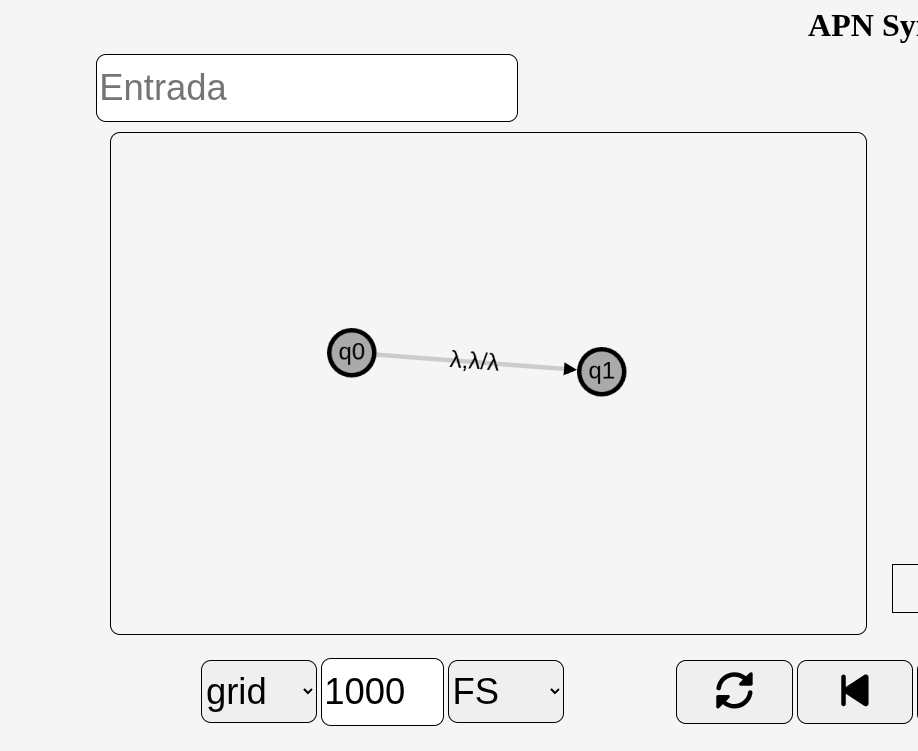
\includegraphics[scale=.24]{img/createTransition.png}
           \caption{}\label{img:createTransition}
        \end{subfigure}
        \begin{subfigure}{0.5\textwidth}
           \centering
           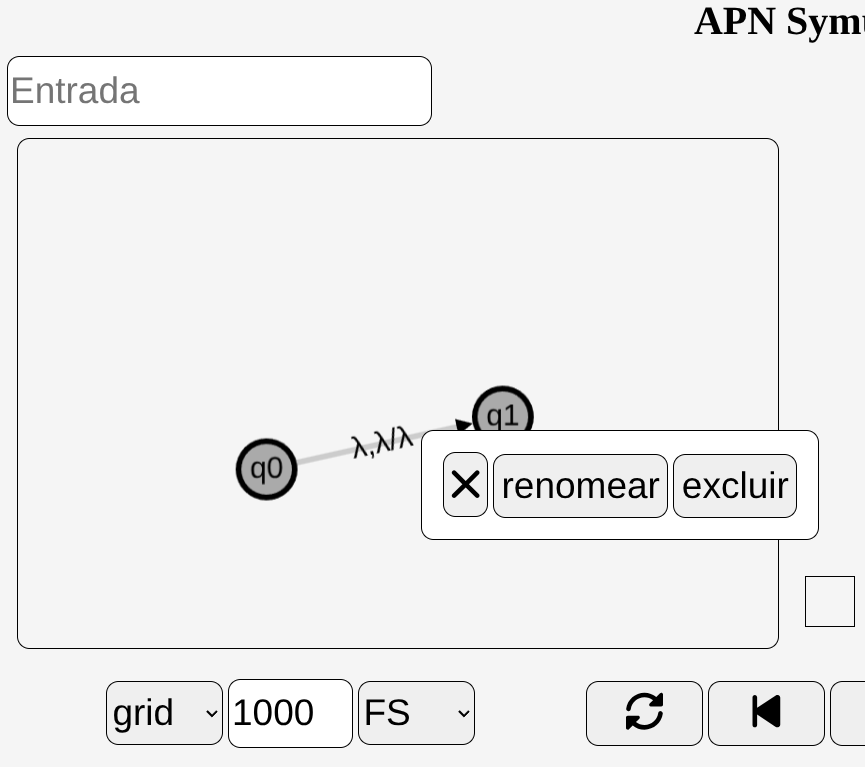
\includegraphics[scale=.24]{img/editTransition.png}
           \caption{}\label{img:editTransition}
        \end{subfigure}
        \caption{\subref{img:createTransition} Criação da transição, \subref{img:editTransition} Editando a transição}
    \end{figure}

    \begin{figure}[h]
        \centering
        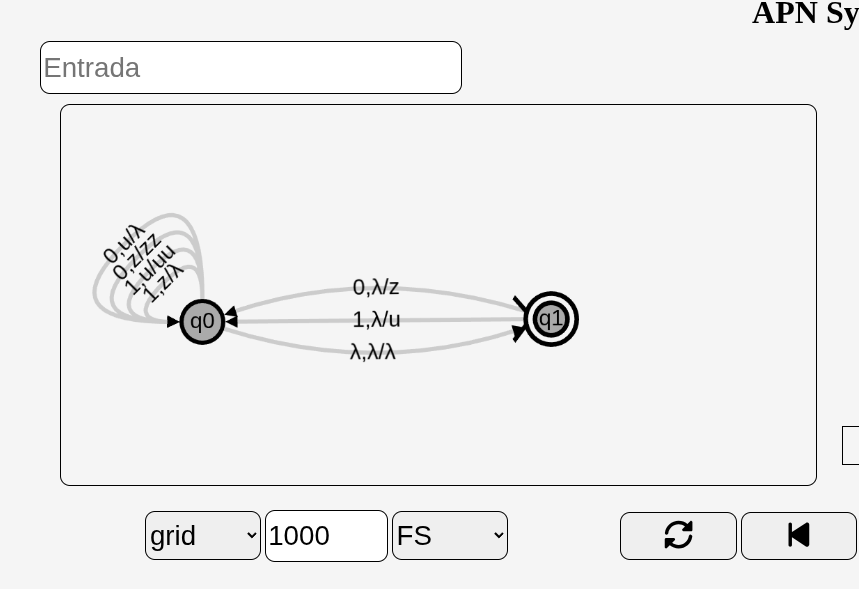
\includegraphics[scale=.24]{img/simpleAPN.png}
        \caption{Um APN simples}
        \label{img:simpleAPN}
    \end{figure}

Ao inserir a palavra de leitura no campo "Entrada" (como a palavra "0101", mostrada na Figura~\ref{img:word0101}) e clicar no botão inferior com ícone de \emph{play}, o sistema calcula a execução completa do autômato. Após clicar no botão com simbolo de \emph{play}, o botão transforma-se no ícone de \emph{stop}, permitindo interromper a demonstração se desejado.

A execução será feita com base em mais dois valores mostrados nessa figura, onde está escrito 1000 está definido o numero maximo de passos de execução que esse automato pode executar antes que a sua parada seja forçada, dado que APNs podem entrar em loop infinito. Além disso existe o seteor onde está escrito FS onde é informado o tipo de aceitação do sistema, sendo, FS estado final e pilha vazia, F apenas vestado final e S apenas pilha vazia. 

    \begin{figure}[h]
        \centering
        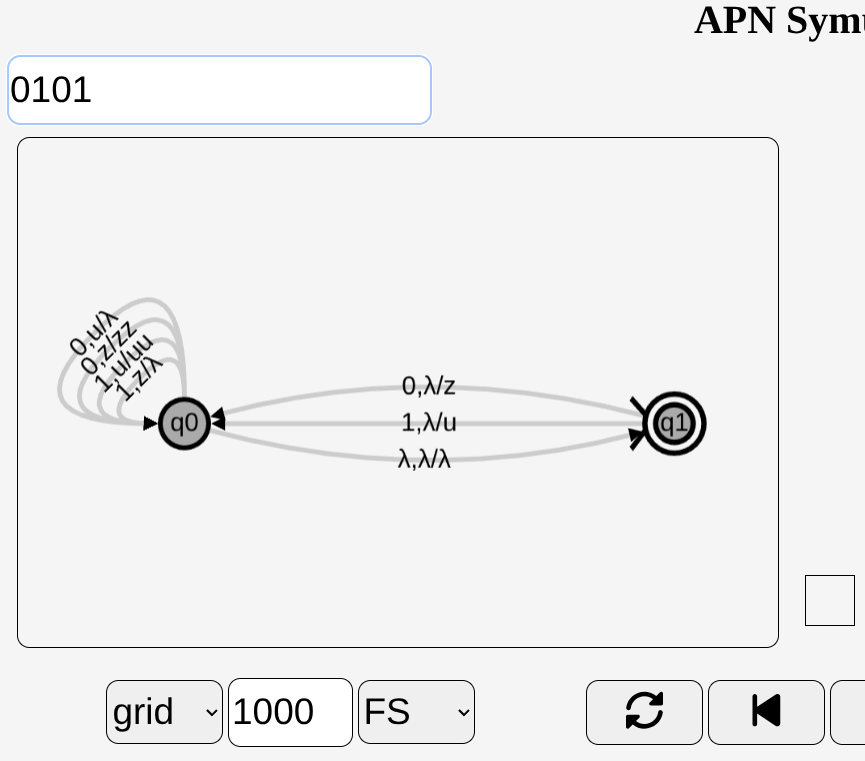
\includegraphics[scale=.24]{img/word0101.png}
        \caption{Entrada da palavra 0101}
        \label{img:word0101}
    \end{figure}

Durante a execução, o campo da palavra é substituído por uma tabela detalhando cada caractere e seu respectivo índice, destacando o último símbolo lido para facilitar a compreensão (Figura~\ref{img:wordTable}). Além disso, no painel direito é possível visualizar as etapas de execução (os \emph{snapshots}). Aqueles associados ao caractere recém-lido são destacados em verde (Figura~\ref{img:snapGraph}). Em cada nó do painel é possível ver: o estado atual na máquina, o índice do caractere lido na palavra e o topo da pilha (até três elementos).

    \begin{figure}[h]
        \begin{subfigure}{0.5\textwidth}
           \centering
           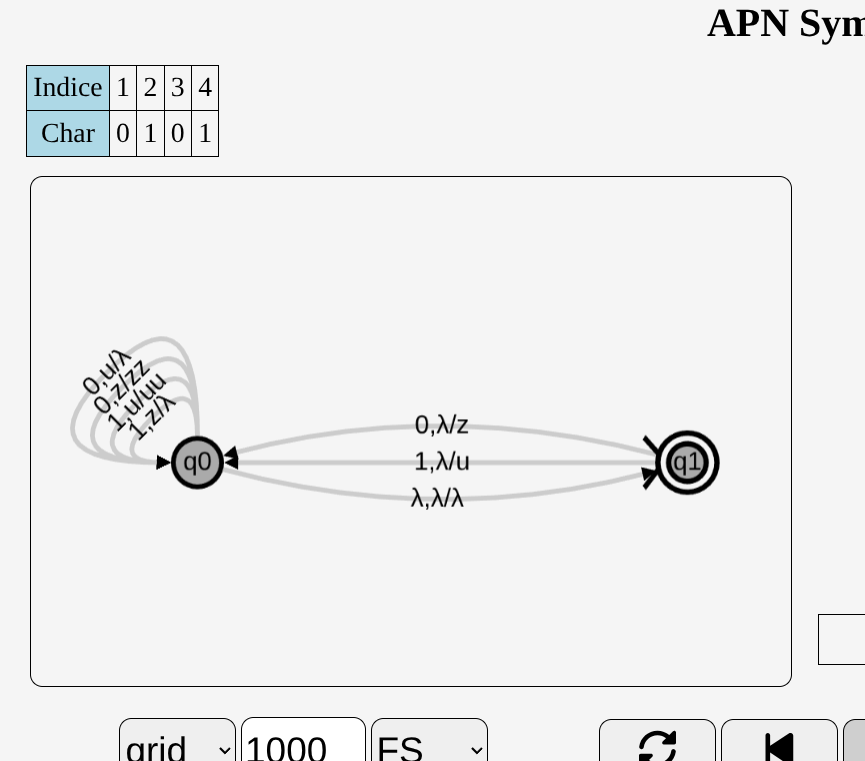
\includegraphics[scale=.24]{img/wordTable.png}
           \caption{}\label{img:wordTable}
        \end{subfigure}
        \begin{subfigure}{0.5\textwidth}
           \centering
           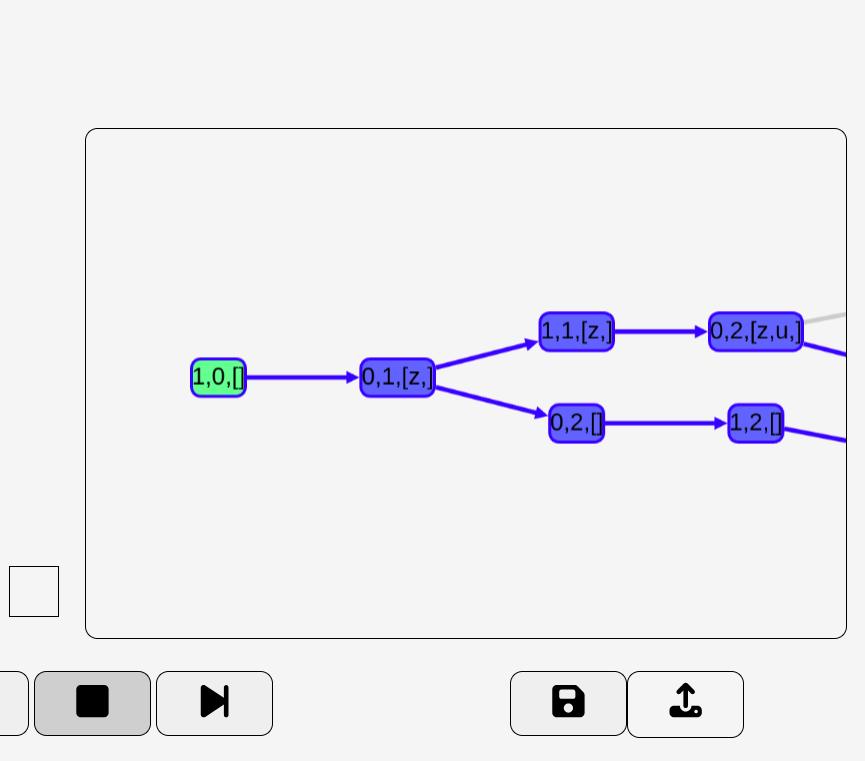
\includegraphics[scale=.24]{img/snapGraph.png}
           \caption{}\label{img:snapGraph}
        \end{subfigure}
        \caption{\subref{img:wordTable} Tabela de caracteres, \subref{img:snapGraph} Visualização dos \emph{snapshots}}
    \end{figure}

No painel direito, as arestas entre os \emph{snapshots} desenhadas em azul indicam os caminhos que podem levar a um estado de aceitação (Figura~\ref{img:acceptedWay}), enquanto as cinzas representam ramos sem sucesso. Ao clicar em um \emph{snapshot}, é possível ver sua pilha completa no centro da tela e visualizar o estado em questão destacado no desenho principal (Figura~\ref{img:snapEfect}). Os botões de avançar e retroceder permitem iterar passo a passo pelo processamento, atualizando os nós em verde (Figura~\ref{img:nextButton}).

    \begin{figure}[h]
        \begin{subfigure}{1\textwidth}
           \centering
           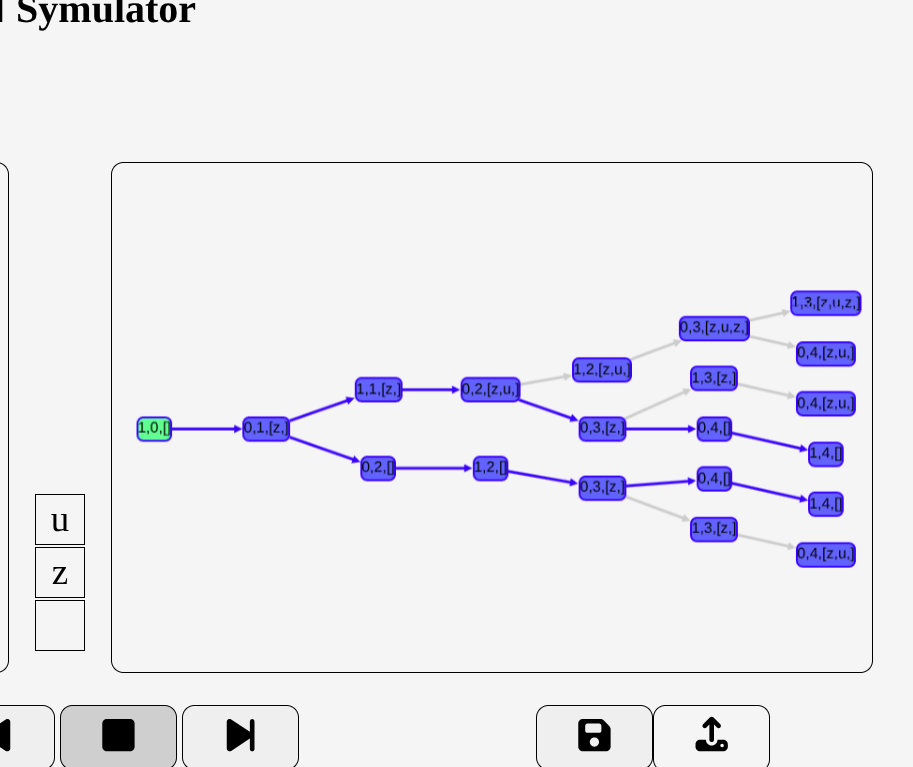
\includegraphics[scale=.24]{img/acceptedWay.png}
           \caption{}\label{img:acceptedWay}
        \end{subfigure}
        \begin{subfigure}{1\textwidth}
           \centering
           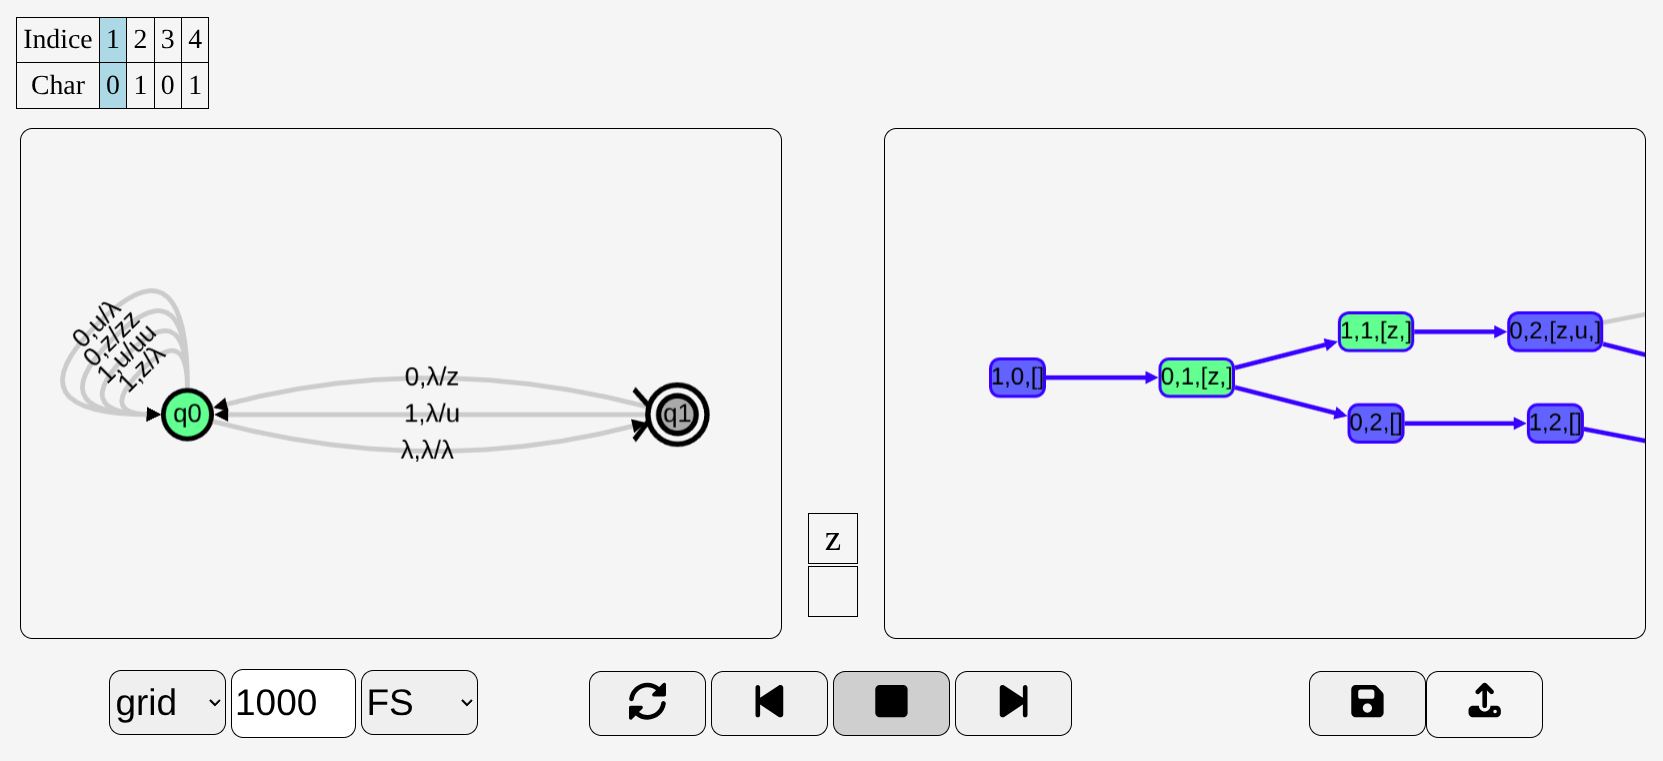
\includegraphics[scale=.24]{img/snapEfect.png}
           \caption{}\label{img:snapEfect}
        \end{subfigure}
        \begin{subfigure}{1\textwidth}
           \centering
           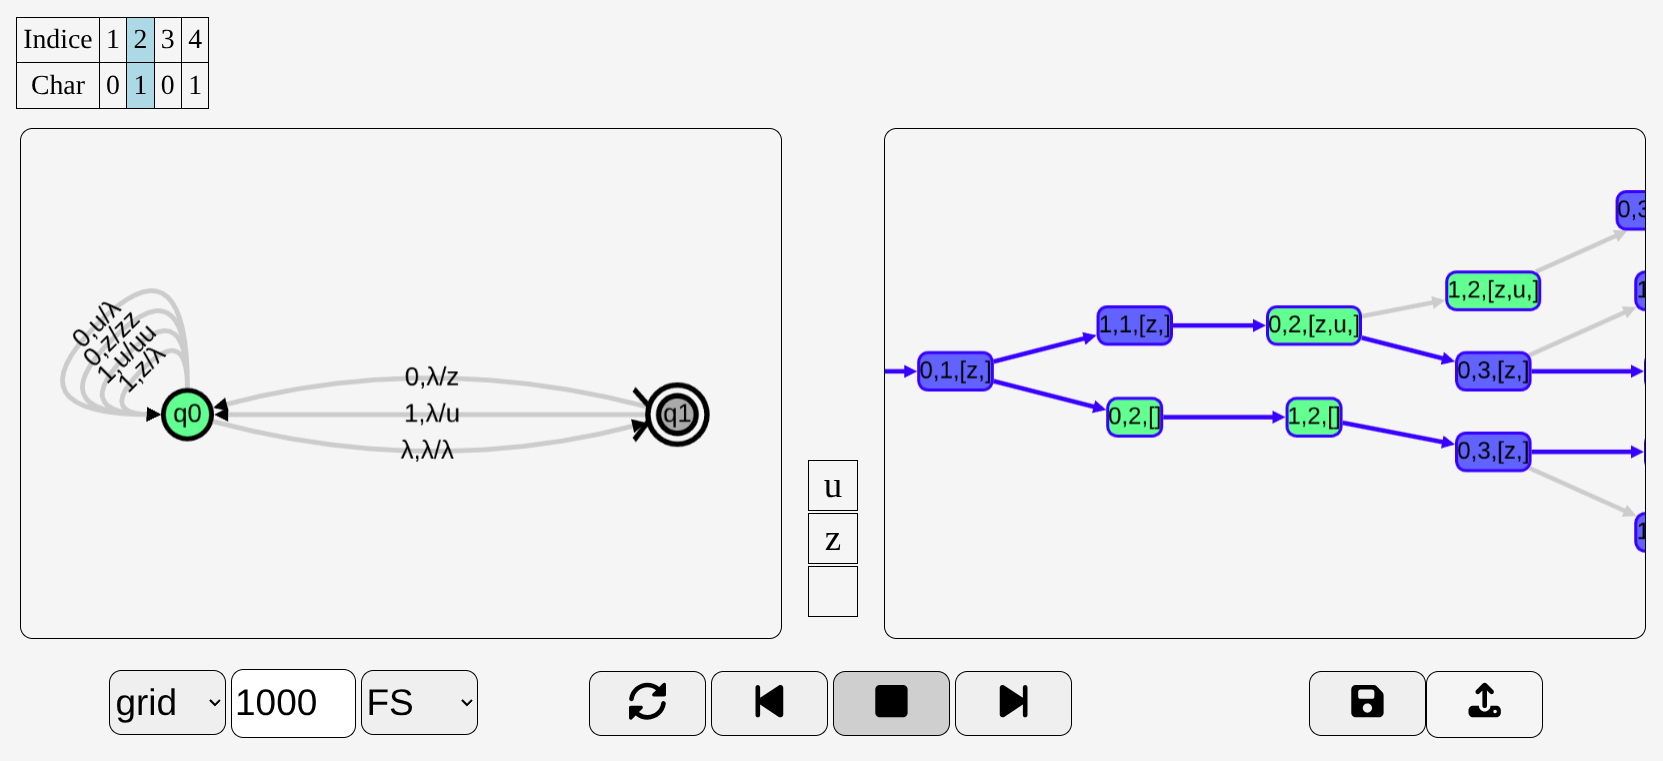
\includegraphics[scale=.24]{img/nextButton.png}
           \caption{}\label{img:nextButton}
        \end{subfigure}
        \caption{\subref{img:acceptedWay} Caminho de aceitação, \subref{img:snapEfect} Clique em \emph{snapshot}, \subref{img:nextButton} Botão de avançar}
    \end{figure}

No canto inferior esquerdo, encontram-se três botões de configuração (Figura~\ref{img:configButtons}): o primeiro ajusta o \emph{layout} visual; o segundo define o limite numérico de \emph{loops} para interromper execuções infinitas; e o terceiro seleciona o critério de aceitação (FS, S ou F). Por fim, no canto inferior direito, há dois botões (Figura~\ref{img:downloadButtons}): o ícone de disquete realiza o \emph{download} do autômato criado em formato JSON, e o ícone de seta faz o \emph{upload} de um JSON contendo uma máquina previamente salva.

    \begin{figure}[h]
        \begin{subfigure}{0.5\textwidth}
           \centering
           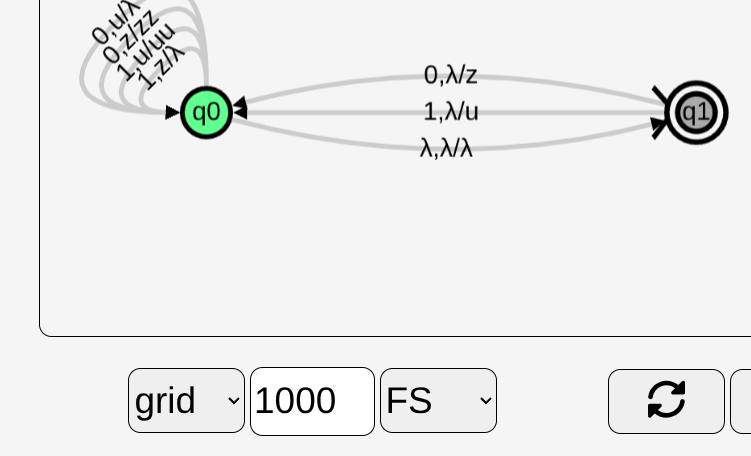
\includegraphics[scale=.3]{img/configButtons.png}
           \caption{}\label{img:configButtons}
        \end{subfigure}
        \begin{subfigure}{0.5\textwidth}
           \centering
           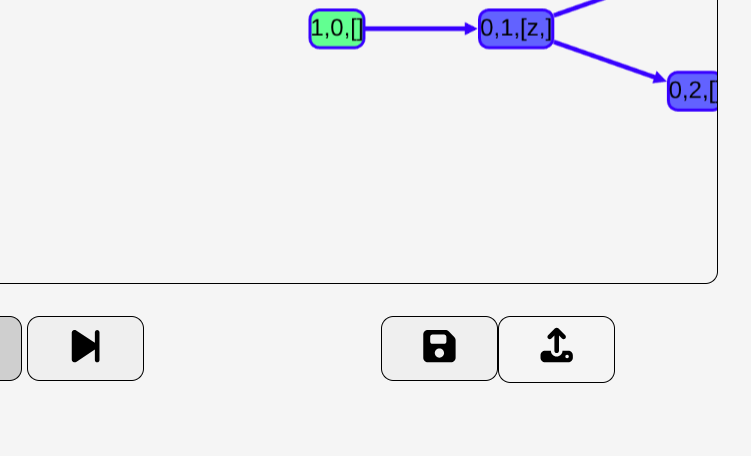
\includegraphics[scale=.3]{img/downloadButtons.png}
           \caption{}\label{img:downloadButtons}
        \end{subfigure}
        \caption{\subref{img:configButtons} Botões de configuração, \subref{img:downloadButtons} Botões de \emph{download}/\emph{upload}}
    \end{figure}
